\section{\textbf{{Visão computacional}}}
\label{visao-computacional}

A visão computacional evoluiu consideravelmente nos últimos anos. Em consequência dessa evolução, a visão computacional se aprimorou a ponto de chegar mais próximo da visão humana, com a capacidade de maior eficiência em várias situações.

A visão computacional abrange todas as técnicas e métodos de processamento de imagem em um único meio, com o objetivo de ser mais eficiente nas análises de dados e informações compostas dentro de uma imagem. \citeonline{SILVA2017} contextualizam que algoritmos de visão computacional utilizam matrizes bidimensionais ou hiperdimensionais como entrada de dados e, a partir desta, produzem informações compactadas como saída.

De forma didática, a área de visão computacional utiliza modelos descritivos de objetos, pessoas e/ou cenas capturadas digitalmente para automatizar processos e realizar tomadas de decisão.

A visão computacional foi desenvolvida, segundo \citeonline{MARR76}, através da neurofisiologia da visão humana (\autoref{fig_visao-humana}). Seu modelo era estabelecido em níveis de compreensões necessárias à computação da visão estereoscópica, ou seja, o modelo é capaz de trabalhar com eficiência no ambiente tridimensional, onde a análise é feita através de duas imagens obtidas em postos diferentes.

\begin{figure}[h]
	\caption{\label{fig_visao-humana}Esquema mostrando imagens captadas em cada olho. Devido à diferença de
ponto de vista, as imagens então captadas são diferentes.}
	\begin{center}
		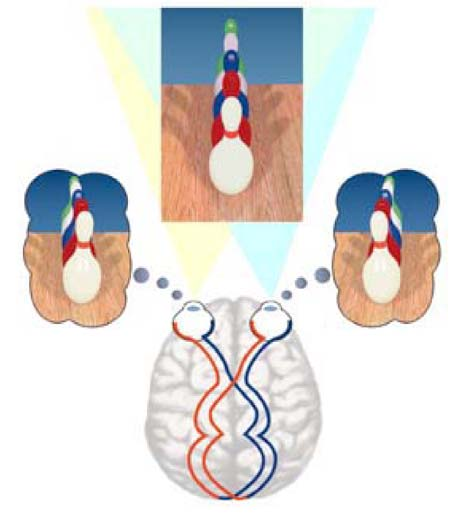
\includegraphics[scale=0.3]{4-Conteudo-Bibliografico/2-Visao-Computacional/Imagens-Visao-Computacional/visao-humana.png}
	\end{center}
	\centering \legend{Fonte: \citeonline{PERONTI2008}}
\end{figure}

\citeonline{PERONTI2008} explica em seu artigo que estereoscopia é a visualização feita por dois mecanismos de captura de imagem em um mesmo foco (\autoref{fig_visao-computacional-camera}).

\begin{figure}[ht]
	\caption{\label{fig_visao-computacional-camera}Mecanismos para captação de imagens com focos visuais coincidentes.}
	\begin{center}
		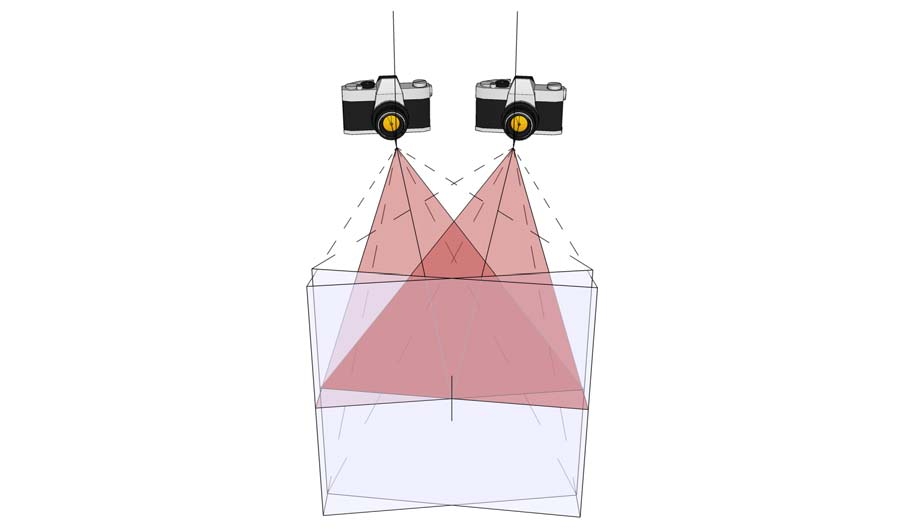
\includegraphics[scale=0.4]{4-Conteudo-Bibliografico/2-Visao-Computacional/Imagens-Visao-Computacional/visao-computacional-camera.png}
	\end{center}
	\centering \legend{Fonte: \citeonline{PERONTI2008}}
\end{figure}

Segundo \citeonline{REHEM2009}, devido ao avanço tecnológico, desenvolveram-se computadores com maior capacidade de processamento gráfico, proporcionando ferramentas com um potencial maior na área de visão computacional. Pode-se dizer que essas ferramentas são bibliotecas onde o seu código fonte é constituído de um agrupamento de funções que potencializam o processamento gráfico de imagens e vídeos. Sendo assim, ao utilizar essas bibliotecas, tem-se a possibilidade de desenvolvimento de técnicas de aperfeiçoamento gráfico para realizar rastreamento de movimentos e de características humanas em tempo real.


\subsection{Captura e identificação de imagem}

A tecnologia vem crescendo cada vez mais em todo mundo, proporcionando a ampliação do uso de dispositivos de alto desempenho. Paralelo a isso, o fluxo de dados aumenta proporcionalmente, exigindo uma velocidade de conexão maior com a Internet. Um exemplo disso são os \textit{smartphones}, que se popularizaram por serem dispositivos multifuncionais, podendo ser utilizados para tarefas profissionais e pessoais. 

Por conseguinte deste avanço científico, é notório a grande evolução na utilização de imagens digitais em várias áreas, como, por exemplo, em transmissões de TV, conteúdos via streaming, imagens capturadas por satélite e até mesmo imagens transmitidas pelas redes sociais. No entanto, como funciona a captura de uma imagem em tempo real? Qual o conceito de imagem?

Uma imagem digital pode ser considerada como sendo uma matriz de pontos elementares, em que cada ponto recebe o nome de \textit{pixel}. Quanto maior a quantidade de \textit{pixels} melhor a resolução da imagem e consequentemente maior o seu tamanho. Cada \textit{pixel} é representado por um valor que indica a intensidade de brilho, denominado nível de cinza, e a quantidade de níveis de cinza depende da quantidade de bits usada na representação de cada \textit{pixel} \cite{SOUZA2007}.

Sendo assim, a matriz de pontos elementares de uma imagem digital pode ser representada conforme na \autoref{fig_imagem-digital-monocromatica}.

\begin{figure}[h]
	\caption{\label{fig_imagem-digital-monocromatica}Representação de uma imagem digital.}
	\begin{center}
		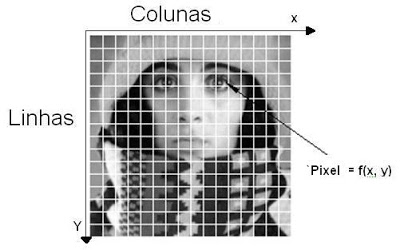
\includegraphics[scale=0.5]{4-Conteudo-Bibliografico/2-Visao-Computacional/Imagens-Visao-Computacional/imagem-digital-monocromatica.JPG}
	\end{center}
	\centering \legend{Disponível em: http://sdbmcc.blogspot.com/2009/06/imagem-digital-teoria.html}
\end{figure}

A captura e identificação em tempo real de uma imagem consiste em analisar um ambiente tridimensional e elaborar digitalmente uma imagem 2-D (Duas dimensões), ocasionando uma imagem estática daquele ambiente tridimensional selecionado. Esse conceito está relacionado a perspectiva, segundo \citeonline{PERONTI2008}. Para que isso seja possível, é necessário utilizar um dispositivo capaz de realizar essa ação, ou seja, uma câmera digital, \textit{smartphones}, dentre outros.

Segundo \citeonline{CHMIELEWSKI2009}, isso se tornou capaz devido a uma tecnologia que surgiu nos anos 70 denominada CCD, \textit{Charge Coupled Device} (Dispositivo acoplado de carga): “O sensor CCD ou dispositivo de carga acoplada é uma matriz de elementos sensíveis à luz, fabricados utilizando tecnologia MOS, \textit{Metal Oxide Semiconductor} (Semicondutor de óxido metálico), onde cada \textit{pixel} pode ser considerado como um capacitor MOS.”

Atualmente, o sensor mais utilizado nos dispositivos de captura de imagem são de sistemas digitais CMOS - \textit{Complementary Metal Oxide Semiconductor} (Semicondutor complementar de óxido metálico), que surgiu nos anos 90 devido a um protótipo do sensor de imagem APS - \textit{Active Pixel Sensor} (Sensor de pixel ativo) criado pela NASA - \textit{National Aeronautics and Space Administration} (Administração Nacional Aeronáutica e Espacial), que possibilitou a fabricação direta de funções como \textit{zoom}, diferentes resoluções de aquisições, acesso aleatório, etc., podendo executar todas as funções do CCD. “Os sensores de imagem APS são formados por elementos sensíveis à luz, capazes de gerar um sinal elétrico ou carga proporcional à intensidade da luz que incide sobre eles.” \cite{CHMIELEWSKI2009}

\subsection{Processamento de imagem}

O grande marco da área de processamento de imagens aconteceu no século XX com o surgimento dos primeiros computadores digitais com grande capacidade de processamento e o início do programa espacial norte-americano, ocorreu um grande impulso na área de processamento de imagem. O uso de técnicas computacionais de aprimoramento de imagens teve início no \textit{Jet Propulsion Laboratory} (Laboratório de Propulsão a Jato), localizado no centro tecnológico da NASA, em 1964, quando "imagens da lua transmitidas por uma sonda Ranger eram processadas por computador para corrigir vários tipos de distorção inerentes à câmera de TV acoplada à sonda". Essa tecnologia foi usada em grandes expedições tripuladas, como a Apollo \cite{FILHO1999}.

Para realizar o processamento de uma imagem, são definidos passos a serem seguidos para a garantia do objetivo final. A captura da imagem consiste no uso de dispositivos físicos sensíveis a espectros de energia eletromagnética que convertem o sinal elétrico para um formato digital. O pré-processamento consiste no realce da imagem para enfatizar características de interesse ou recuperar imagens que sofreram alguma degradação devido à introdução de ruído, perda de contraste ou borramento. A segmentação é a extração ou identificação dos objetos contidos na imagem, separando a imagem em regiões. Por fim, a classificação, é o processo que identifica a imagem observada \cite{GONZALEZ2002}.

As etapas básicas do processamento de imagem estão representadas através da \autoref{fig_etapas-processamento-imagem}.

\begin{figure}[h]
	\caption{\label{fig_etapas-processamento-imagem}Etapas básicas do processamento de imagens.}
	\begin{center}
		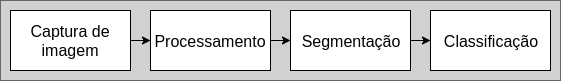
\includegraphics[scale=0.7]{4-Conteudo-Bibliografico/2-Visao-Computacional/Imagens-Visao-Computacional/etapas-processamento-de-imagem.png}
	\end{center}
	\centering \legend{Fonte: Adaptada de \citeonline{GONZALEZ2002}}
\end{figure}

Seres humanos conseguem distinguir vários padrões de cores com certa facilidade, levando em consideração que a análise é feita em um ambiente tridimensional. Na computação, esse discernimento de cores são mais complexos, independentemente da dimensão na qual a imagem será analisada. Isso ocorre porque vários fatores podem contribuir para a má performance computacional no tratamento da imagem, como por exemplo a falta ou excesso de luz, qualidade do sensor, qualidade da imagem, dentre outros.

\begin{citacao}
“Objetos que emitem luz visível são percebidos em função da soma das cores espectrais emitidas. Tal processo de formação é denominado aditivo. O processo aditivo pode ser interpretado como uma combinação variável em proporção de componentes monocromáticas nas faixas espectrais associadas às sensações de cor verde, vermelho e azul, as quais são responsáveis pela formação de todas as demais sensações de cores registradas pelo olho humano. Assim, as cores verde, vermelho e azul são ditas cores primárias. Este processo de geração suscitou a concepção de um modelo cromático denominado RGB (Red, Green, e Blue), para o qual a Comissão Internacional de Iluminação (CIE) estabeleceu as faixas de comprimento de onda das cores primárias.” \cite{QUEIROZ2006}
\end{citacao}

Cada \textit{pixel} é representado por um valor numérico que corresponde a sua cor em questão. Sendo assim, para que seja possível representar uma imagem em alguma escala de cor monocromática (preto e branco, ou escalas de cinza), basta associar o \textit{pixel} a um valor numérico relacionado a sua escala de tom.

A \autoref{fig_rep-pixel-monocromatico} exemplifica a associação dos \textit{pixels} de forma a obter uma imagem monocromática. Segundo \citeonline{NELMA2000}, para obter uma imagem em tons de cinzento, basta associar cada \textit{pixel} um valor inteiro não negativo de um byte, onde o valor 0 corresponde a cor preta e o valor máximo, 255, corresponde a cor branca. Os valores intermediários correspondem aos variados tons de cinza.

\begin{figure}[h]
	\caption{\label{fig_rep-pixel-monocromatico}Imagem médica digital em escalas de cinza (\textit{pixels} monocromáticos).}
	\begin{center}
		\resizebox{.8\linewidth}{!}{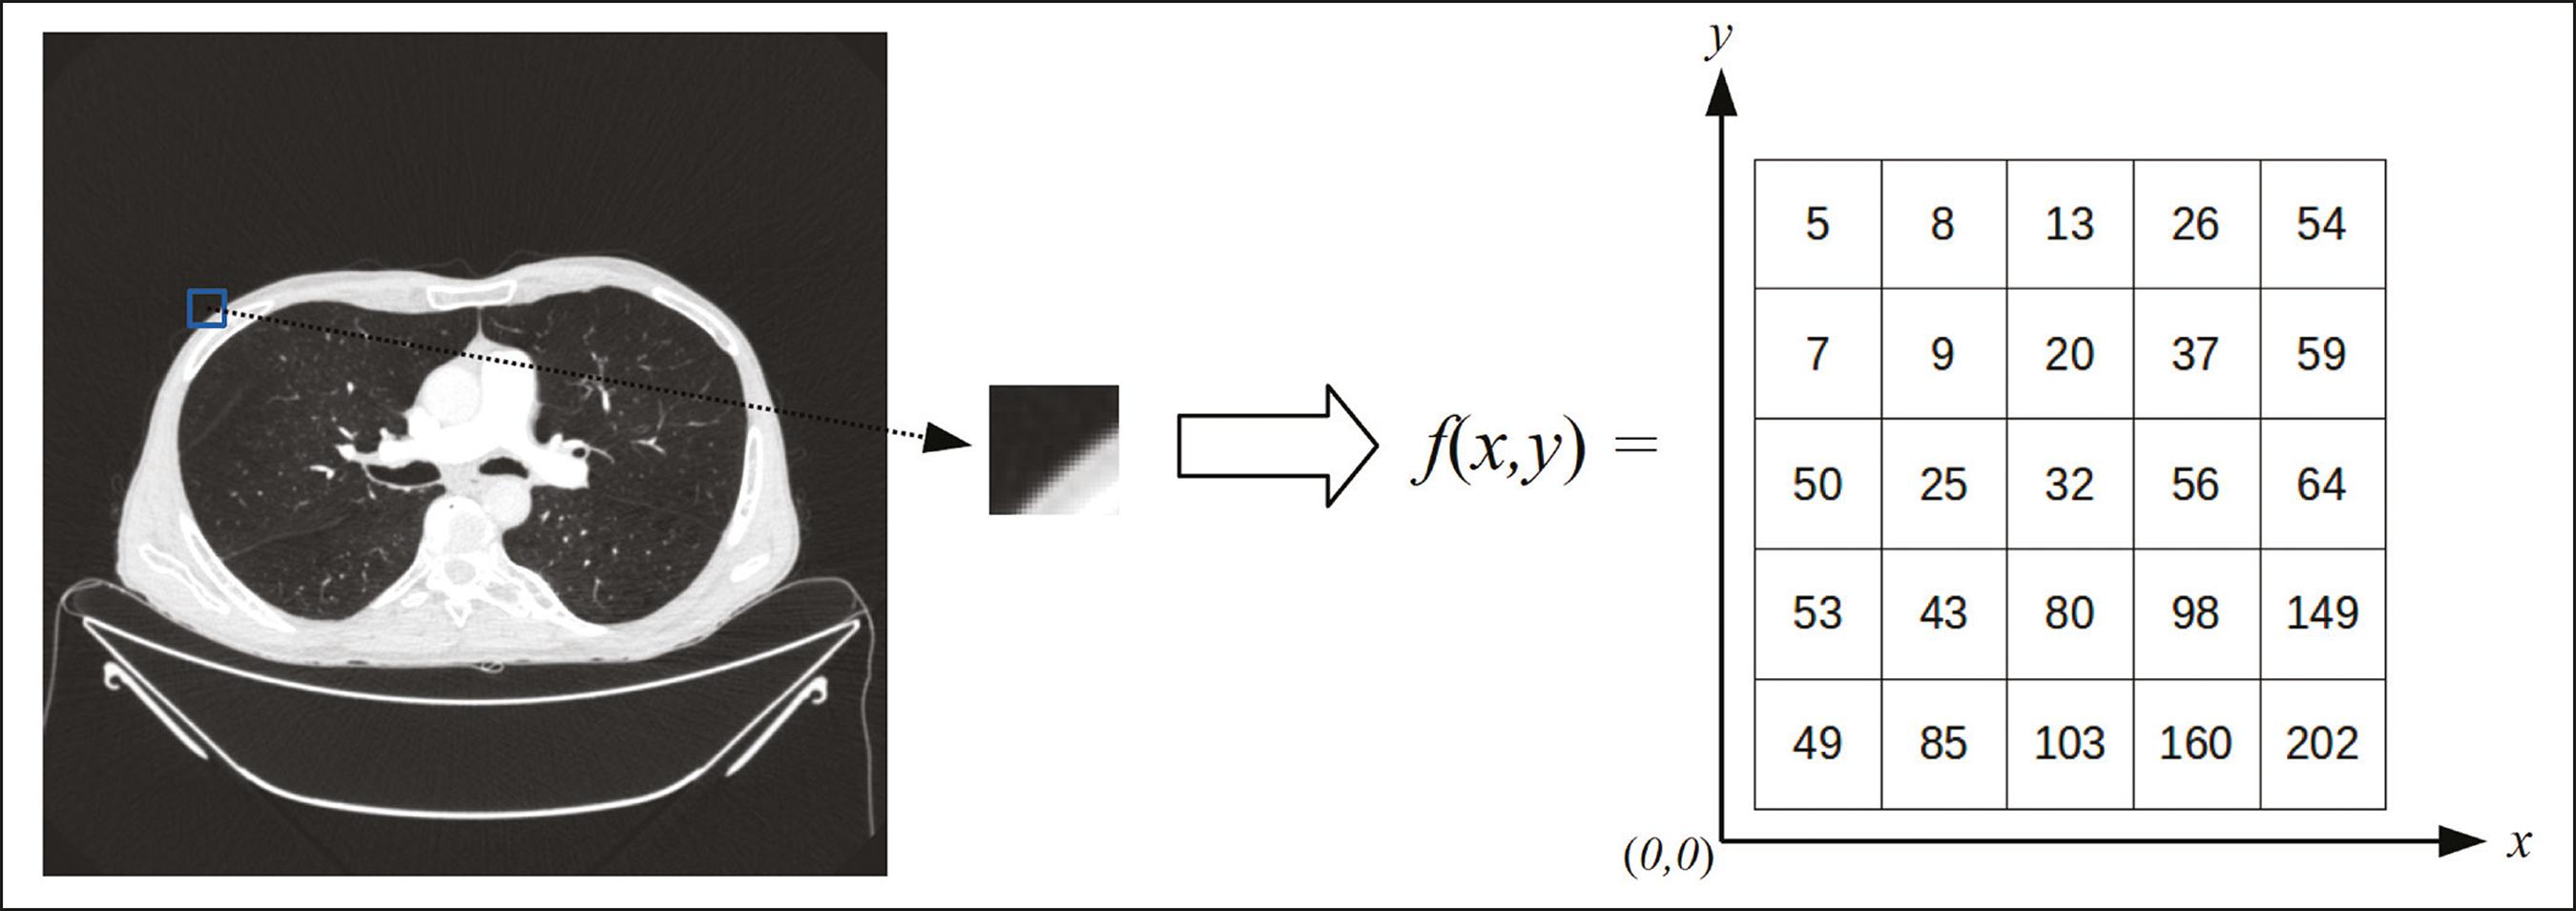
\includegraphics{4-Conteudo-Bibliografico/2-Visao-Computacional/Imagens-Visao-Computacional/repr-pixel-monocromatico.jpg}}
	\end{center}
	\centering \legend{Fonte: \citeonline{SANTOS2019}}
\end{figure}

Já as imagens coloridas exigem um poder maior de processamento para serem reconhecidas. Isso ocorre porque as imagens em RGB - \textit{Red, Green, and Blue} (Vermelho, Verde e Azul)  precisam de mais de uma banda\footnote{Cada matriz ou conjunto de cor diferente é denominado banda de cor. Subconjuntos de três bandas espectrais azul, vermelha e verde compõem uma imagem RGB. Em imagens monocromáticas (Preto e branco), o objeto é representado em apenas uma banda espectral \cite{CROSTA1999}. \label{Banda-de-Cor}} para serem processadas, ou seja, são analisadas três matrizes de cores para formar a paleta de cor específica do tom capturado (\autoref{fig_rgb-representacao}). Depois da análise, são formadas as cores distintas que compõe a imagem.

\begin{figure}[h]
	\caption{\label{fig_rgb-representacao}Matriz de \textit{pixels} RGB.}
	\begin{center}
		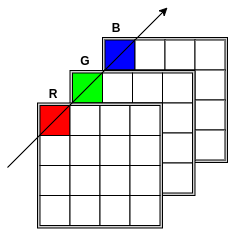
\includegraphics[scale=0.6]{4-Conteudo-Bibliografico/2-Visao-Computacional/Imagens-Visao-Computacional/matriz-de-pexels-rgb.png}
	\end{center}
	\centering \legend{Fonte: Elaborada pelos autores do projeto.}
\end{figure}

De forma mais detalhada, \citeonline{LOPES2013} exemplificam que imagens coloridas também são imagens multibanda, ou multiespectral. As cores visíveis através de olhos humanos podem ser representadas pela combinação de bandas das cores primárias vermelha, verde e azul (\textit{Red, green} e \textit{blue}, respectivamente). A imagem colorida também pode ser armazenada por meio de imagens cromáticas e mapas de cores. Nesse caso, o valor de cinza de cada \textit{pixel} na imagem se torna um índice para uma entrada de mapa de cores, enquanto a entrada em si do mapa de cores contem os valores dos componentes referentes as tonalidades \textit{RGB} (\autoref{fig_rep-pixel-rgb}).

\begin{figure}[h]
	\caption{\label{fig_rep-pixel-rgb}Imagem digital em tons coloridos (\textit{pixels} RGB).}
	\begin{center}
		\resizebox{.6\linewidth}{!}{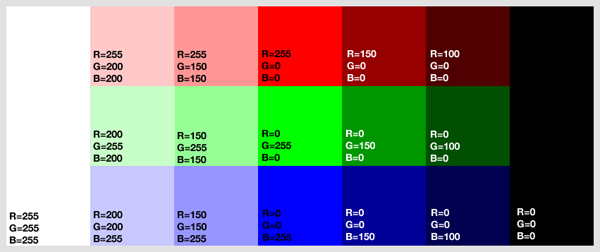
\includegraphics{4-Conteudo-Bibliografico/2-Visao-Computacional/Imagens-Visao-Computacional/repr-pixel-rgb.jpg}}
	\end{center}
	\centering \legend{Disponível em: https://apenasimagens.com/pt/pixel-imagem-digital/}
\end{figure}

No entanto, a imagem capturada por algum dispositivo eletrônico pode chegar de forma irregular ate a parte de processamento. Essas falhas podem ser caracterizadas de várias formas, como por exemplo a presença de \textit{pixels} ruidosos, brilho e/ou contrastes desregulados, caracteres com dígitos incompletos ou apagados como em digitalizações de documentos.

A parte de processamento fica responsável por elaborar uma melhoria da imagem em questão, ajustando todos os parâmetros para que seja possível analisar precisamente todas as informações que estão disponíveis no arquivo de imagem. Sendo assim, por analogia as imagens processadas, trata-se de uma etapa que analisa de forma profunda todos os dados contidos na imagem, ou seja, a fase de processamento abrange os níveis mais baixos de análise de imagens, pois trabalham diretamente com valores de intensidade dos \textit{pixels}, visto que neste período não existe nenhuma informação relacionada a imagem para que seja possível facilitar o trabalho.

\subsubsection{\textit{Segmentação de imagens}}

De forma a dar continuidade ao ciclo de processamento de imagem e verificação desta, usa-se métodos de \textit{pixels} e tonalidades seguindo os padrões propostos. A análise deve prosseguir de forma minuciosa para então, processar seus detalhes.

A segmentação veio para aprimorar a parte de processamento, auxiliando na detecção de maiores detalhes e reduzindo tempo de processamento. Isso ocorre porque a segmentação é a área que tem por responsabilidade dividir a imagem em várias partes significativas, separando as de interesse dentro desta \cite{FILHO1999}.

No entanto, a segmentação exige um processamento muito grande para analisar a imagem sugerida. Sendo assim, o nível no qual será feito essa subdivisão de imagem depende muito da ocasião e do problema que está sendo proposto para resolver. De acordo com \citeonline{GONZALEZ2002}, para não ocorrer perca desnecessária de processamento e, consequentemente, perda de tempo, a segmentação deve parar assim que os objetos de interesse da aplicação forem isolados.

Portanto, dentro da segmentação existem métodos que podem ser seguidos a fim de analisar detalhadamente cada figura. Segundo \citeonline{MORGAN2008}, as classificações dos métodos utilizados na segmentação são definidos como interativos ou automáticos. Basicamente, a diferença entre os dois são bem simples: um é executado através de intervenções humanas e o outro não.

Além disso, no processo de segmentação interativa, o usuário utiliza ferramentas e técnicas que se adéquam da melhor forma a sua imagem e necessidade, solucionando-a da melhor forma possível. Esse método normalmente é mais utilizado para solucionar problemas específicos, onde as condições da imagem podem interferir drasticamente na análise final da mesma como, por exemplo, \textit{softwares} que analisam imagens de doenças graves adquiridas através de ressonâncias, onde a aplicação pode confundir um ruído ou uma área com má iluminação em um ponto de análise clínica.

Já o processo de segmentação automática onde, na maioria das vezes, utilizam robôs para realizar as tomadas de decisões através dos resultados obtidos na análise da imagem, inexiste interferência humana no processo. Esse método está sendo aplicado, por exemplo, em carros autônomos, onde o mesmo identifica a presença de obstáculos em sua frente e com base no obstáculo e na proporção do mesmo, uma ação e tomada.

Para complementar, \citeonline{MORGAN2008} enfatiza que existem métodos que são classificados de acordo com a representação dos objetos a serem segmentados, que são os métodos de borda ou orientados a regiões.

O processo de segmentação baseado no método de bordas utiliza basicamente pontos de uma imagem onde ocorre alguma intensidade de luz, ou seja, onde os \textit{pixels} estão mais visíveis, realçando a borda do objeto e consequentemente diferenciando do fundo da imagem. Pode-se também localizar uma borda através de uma mudança brusca nos tons de cinza, gerados por regiões distintas. Com base na borda que foi extraída da imagem, tem-se então uma imagem topográfica do objeto que será analisado.

A \autoref{fig_metodo-de-borda} mostra como funciona uma análise baseada no método de bordas.

\begin{figure}[h]
	\caption{\label{fig_metodo-de-borda}Resultado de uma análise feita utilizando o método de bordas.}
	\begin{center}
		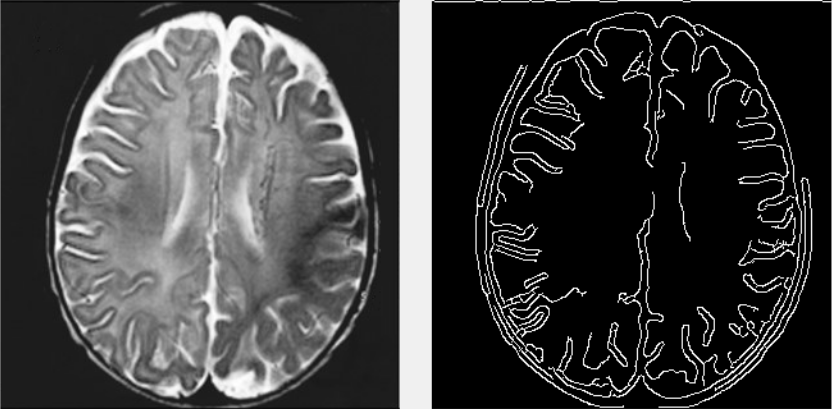
\includegraphics[scale=0.3]{4-Conteudo-Bibliografico/2-Visao-Computacional/Imagens-Visao-Computacional/metodo-de-borda.png}
	\end{center}
	\centering \legend{Fonte: \citeonline{FREITAS2016}}
\end{figure}

Conforme \citeonline{MORGAN2008} enfatiza em seu artigo, o método orientado a regiões é dividido em três abordagens relevantes: classificação por \textit{pixel}, agregação de \textit{pixel} e \textit{split-and-merge} (Divisão e conquista).

A descrever cada uma das abordagens de forma didática, a classificação por \textit{pixel} nada mais é que a identificação de características presentes na imagem como, por exemplo, cor, texturas, a fim de classificar os \textit{pixels} de acordo com as várias possibilidades de classes ou objetos da imagem.

Na abordagem de agregação por \textit{pixel} o objetivo é encontrar um \textit{pixel} dentro da imagem e, a partir desse \textit{pixel}, ocorre o crescimento de regiões conexas. O desenvolvimento das regiões acontece ate alcançar o critério de parada do crescimento, onde estará representado um objeto dentro da imagem.

Já a segmentação utilizando a bordagem \textit{split-and-merge} é mais complexa. Segundo \citeonline{VENTURA2009}, ao aplicar essa abordagem de segmentação, o objetivo final consiste em conseguir subdividir a imagem em vários quadrantes que satisfaça uma prioridade. Apos a concretização desta tarefa, realiza-se a verificação de cada quadrante, observando se este atende ou não a prioridade definida. Caso o quadrante não satisfaça a prioridade, a subdivisão acontece novamente em busca de outros quadrantes.

Por fim, o processo de fusão é realizado, acontecendo então o agrupamento das partes similares, ou seja, que atende as prioridades definidas. Esse processo só finaliza quando não existe nenhuma possibilidade de realizar divisões ou agrupamentos.

\subsubsection{\textit{Histograma}}

O histograma é um método que auxilia na identificação de objetos e/ou características específicas da imagem, obtendo uma maior precisão nos resultados obtidos.

Segundo \citeonline{FILHO1999}, histogramas são conjuntos de vários números no qual são indicados os percentuais de \textit{pixels} de uma imagem que possui determinados níveis de cinza. Estes valores, normalmente representados por gráficos, apresentam, para cada nível de cinza, o seu percentual de \textit{pixels} correspondente na imagem. Com base nessa análise feita pelo histograma, pode-se obter os níveis de contraste, brilho, e até mesmo informações de predominância clara ou escura.

\citeonline{FILHO1999} explicam que, através de equações matemáticas, é possível obter um resultado satisfatório ao analisar cada elemento deste conjunto. Este trabalho não tem por finalidade apresentar e/ou explicar cálculos matemáticos que cada função executa.

De forma a complementar o assunto, \citeonline{MAIZA2013} expressa em sua tese que, ao obter o histograma da imagem, pode-se alcançar medidas estatísticas dos níveis de cinza da imagem, como por exemplo o seu valor mínimo e máximo, valor médio, variância e desvio padrão. Portanto, o histograma seria como um método de probabilidade, onde o número de \textit{pixels} de um determinado nível de cinza pode ser utilizado para calcular um outro \textit{pixel} com o mesmo valor de cinza na imagem (\autoref{fig_histograma}).

\begin{figure}[h]
	\caption{\label{fig_histograma}Imagem (a) e seu respectivo histograma (b).}
	\begin{center}
	\resizebox{.8\linewidth}{!}{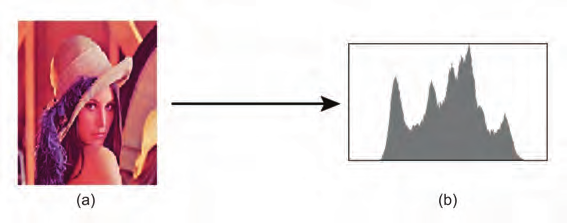
\includegraphics{4-Conteudo-Bibliografico/2-Visao-Computacional/Imagens-Visao-Computacional/histograma.png}}
	\end{center}
	\centering \legend{Fonte: \citeonline{MAIZA2013}}
\end{figure}

\subsubsection{\textit{Classificação de imagens}}
\label{classificacao-de-imagem}
% \textbf coloca o subsection em negrito

A classificação de imagem é a última etapa do processamento de imagem (\autoref{fig_etapas-processamento-imagem}). Em síntese, esta etapa é responsável por realizar a classificação das imagens levando em consideração as suas características.

Entretanto, segundo \citeonline{LIBERMAN97}, nessa etapa do processamento, o grau de abstração de cada característica da imagem pode ser classificado em três níveis distintos: baixo, médio e alto.

No processo de baixo nível são utilizados os \textit{pixels} originais da imagem como parâmetros de comparação, para que no final do processo sejam gerados propriedades da imagem, em forma de valores numéricos, associadas a cada \textit{pixel} que foi analisado. Sequencialmente, o nível médio coleta essas propriedades numéricas geradas pelo processo de baixo nível e produz uma lista de características da imagem. Por fim, o processo de alto nível reúne estas características ocasionadas pelo processo anterior buscando interpretá-las, formando assim o conteúdo da imagem.

Segundo \citeonline{LIBERMAN97}, o processo de classificação ou interpretação de uma imagem é a parte mais inteligente da visão computacional. O autor do artigo cita que essa é uma das etapas de maior nível, no qual permite-se obter a “compreensão e a descrição final do fenômeno inicial”.

Para complementar, \citeonline{LIBERMAN97} explica que o processo de classificação de imagem possui duas técnicas para realizar suas tarefas, sendo divididas em supervisionada ou não-supervisionada. A classificação não-supervisionada consiste em um agrupamento automático de sequências similares de uma imagem analisada. Conforme já prescrito neste trabalho no contexto de segmentação interativa e agora completado por \citeonline{LIBERMAN97}, nessa etapa a imagem será segmentada em um número indeterminado de classes, no qual o usuário também será responsável por gerenciar essas classes a fim de alcançar seus objetivos.

De acordo com \citeonline{MAXIMO2005}, no processo de classificação supervisionada, o analista ou usuário filtra as classes de informações seguindo os seus padrões de interesse e separa, na imagem, as regiões que satisfazem essas classes. Após a delimitação das classes, a técnica analisará as mesmas com o objetivo de delimitar \textit{pixels} que serão utilizados como parâmetros para a busca de demais \textit{pixels}.

Simplificadamente, a técnica de classificação supervisionada utiliza amostras de características coletadas durante o processo para identificar cada \textit{pixel} definido como \textit{pixel} desconhecido, ou seja, tons de \textit{pixels} que não fazem parte das características já coletadas anteriormente seguindo os filtros definidos pelo usuário.

\begin{itemize}
\raggedright \item \textit{Haar Cascade}
\end{itemize}
 
Para complementar o assunto citado acima, a técnica de \textit{Haar Cascade} utiliza a classificação de imagens para obter um padrão de características que foram extraídas da imagem. Essa classificação é utilizada para montar uma cascata de características, ou seja, um conjunto de imagens. A principal base para a detecção de objetos do classificador \textit{Haar} são os recursos extraídos da imagem, ou seja, ao invés de usar os valores de intensidade de um \textit{pixel}, usa-se as alterações nos valores de contraste entre os grupos retangulares dos \textit{pixels}. Basicamente, \textit{Haar Cascade} é baseada em \textit{Haar Wavelets}, que utiliza uma sequência de funções redimensionadas em quadrantes que juntas formam uma base de \textit{wavelets} \cite{WILSON2006}.

A detecção de objetos e faces utilizando técnicas de classificadores em cascata baseados em recursos \textit{Haar} é um método eficaz proposto por \citeonline{VIOLA2001} em seu artigo. Á abordagem é baseada em \textit{machine learning} (aprendizado de máquina) no qual a função cascata é treinada a partir de enumeras imagens positivas e negativas. Através desse recurso, pode-se obter a eficiência em detecção de objetos em outras imagens \cite{OpenCV}. Este trabalho não descreve os detalhes do funcionamento do detector de Viola-Jones. O leitor interessado pode encontrá-lo em \cite{VIOLA2001}.

\begin{itemize}
\raggedright \item \label{itm:machinelearning} \textit{Machine Learning}
\end{itemize}

O \textit{haar cascade} pode ser descrito com uma técnica utilizada para gerar um conjunto com todas as características da imagem.  Portanto, é possível utilizar o \textit{machine learning} para obter melhores resultados, porque ele utiliza como parâmetro de entrada o conjunto de características para ajustas e adaptar todos os pontos de interesse do conjunto.  Após a análise do algoritmo, o reconhecimento de imagem pode ser aprimorado. O reconhecimento de padrões e o \textit{machine learning} são técnicas que passaram por um crescimento substancial ao longo dos tempos \cite{BISHOP2006}.
 
Sendo assim, o \textit{machine learning} pode ser definido como a área que estuda alternativas para fazer as máquinas executarem tarefas que se aproximam das atividades humanas. Essa tecnologia possibilitou a criação de sistemas capazes de realizar várias atividades de forma automatizada, ou seja, a tecnologia pode ser programada para realizar tomada de decisões a partir dos dados que são utilizados para treinar o algoritmo \cite{MONARD2003}.

Devido ao crescimento exponencial do aprendizado de máquina, diversos sistemas foram criados para resolver problemas. Isso não significa que existe todos os modelos já feitos para resolver todo o tipo de problema existente. Sendo assim, é necessário entender a capacidade e as limitações da tecnologia para analisar a sua usabilidade, pois seu uso requer muito poder de processamento.

\subsubsection{\textit{Similaridade}}

De forma concisa, similaridade consiste em realizar uma buscar dentro de uma imagem específica com o objetivo de reconhecer/encontrar objetos semelhantes a um modelo de busca. Nessas funções de busca por similaridade são utilizados cálculos de vetores de características para realizar as comparações de igualdade \cite{MAIZA2013}.

Os seres humanos possuem uma grande facilidade de reconhecer informações apresentadas de maneira visual, onde consequentemente são capazes, com grande facilidade, de interpretar imagens diversificadas sem grande esforço. Exemplificando esta situação, os seres humanos consegue distinguir de forma fácil a diferença entre um círculo grande e um círculo pequeno, um quadrado grande de um quadrado pequeno, a diferença entre um triângulo e um quadrado de tamanhos idênticos, dentre outros. Conforme \citeonline{SILVA2009} relata em seu artigo, com a tecnologia disponível atualmente para realizar a construção de aplicações capazes de identificar informações dentro de uma imagem ainda é muito ineficiente, quando comparada com a capacidade humana.

Segundo \citeonline{MAIA2013}, algoritmos de similaridade trabalham com métricas que informam o quanto uma imagem é parecida com a outra. Ou seja, pode-se aplicar essas métricas utilizando padrões de buscas a fim de uma análise mais específica. De forma estatística, \citeonline{MAIA2013} completam que possui dois tipos básicos de medidas de similaridade: correlação e coseno. Seguindo o contexto do artigo, a similaridade por correlação entre dois vetores retorna um valor booleano, ou seja, 0 e 1, onde o valor de retorno igual a 1 significa que há uma similaridade forte naquele ponto, ou seja, os valores dos vetores são parecidos e, se o retorno for 0, não existe correlação. No entanto, o autor enfatiza a presença de um retorno igual a -1, no qual a similaridade daquele ponto é inversa ao padrão de busca. Ja a similaridade por coseno é similar a correlação, no qual o retorno também e 0 e 1, porém nesse método é analisado o tamanho do vetor e a formação de um ângulo entre os mesmos. Quanto mais próximo de 1 for o valor, mais similares são os vetores.

\citeonline{MAIZA2013}, \citeonline{MAIA2013} utilizam em seus artigos a função euclidiana para realizar cálculos de distâncias nas estruturas. Essa função utiliza métricas de similaridade para calcular a distância entre dois vetores de características, percorrendo o vetor apenas uma vez. A distância euclidiana entre dois pontos (Xi e Xj) é definida através de uma equação matemática, na qual não faz parte do escopo deste projeto.

\subsection{Reconhecimento facial}

Dentre as diversas tarefas que os computadores podem executar, o reconhecimento facial tem tido uma crescente, se tornando alvo de vários estudos. Algoritmos de reconhecimento facial estão presente em diversos dispositivos, como por exemplo \textit{smartphones} e câmeras digitais, e ate mesmo carros autônomos, que escaneiam seus obstáculos para realizar uma tomada de decisão. Grandes aperfeiçoamentos dentro desta área estão sendo implementados de forma gradativa com a finalidade de realizar análises com grandes precisões e mais próximas a visão humana.

Segundo \citeonline{SZELISKI2010}, a área de reconhecimento facial foi a que teve mais sucesso nos dias atuais. No entanto, a aplicação desse algoritmo para realizar a busca de uma pessoa dentro de milhares de pessoas em tempo real, ainda é um desafio para a tecnologia, embora pra humanos essa tarefa também é bem difícil. Mas quando esse grupo de pessoas é reduzido a, por exemplo, um grupo familiar ou grupo de amigos, a ferramenta tem um desempenho excepcional. O objeto na qual esta sentá sendo utilizado para ler o ambiente físico, ou seja, o dispositivo de captura de imagem, influencia diretamente com o desempenho da ferramenta.

Sendo assim, o resultado do reconhecimento facial pode ser intensificado quando a imagem é capturada de forma frontal as pessoas, no qual seja possível localizar por completo os rostos das pessoas em questão. Porem, vários fatores podem interferir na análise da imagem, por exemplo: iluminação, qualidade dos sensores, dentre outros fatores de interferência. Para tentar solucionar esses problemas, uma das primeiras abordagens a ser seguida pela ferramente e tentar analisar os locais de características específicas da imagem como, por exemplo, nariz, boca, olhos, e aplicar medidas de distância entre os pontos de características encontrados \cite{SZELISKI2010}.

Existem várias ferramentas que proporcionam ao usuário utilizar a tecnologia de visão computacional para realizar o reconhecimento facial. Dentre estas ferramentas, a biblioteca OpenCV disponibiliza funções capazes de reconhecer objetos e pessoas. 